\chapter{Demonstration slides}

\begin{figure}
    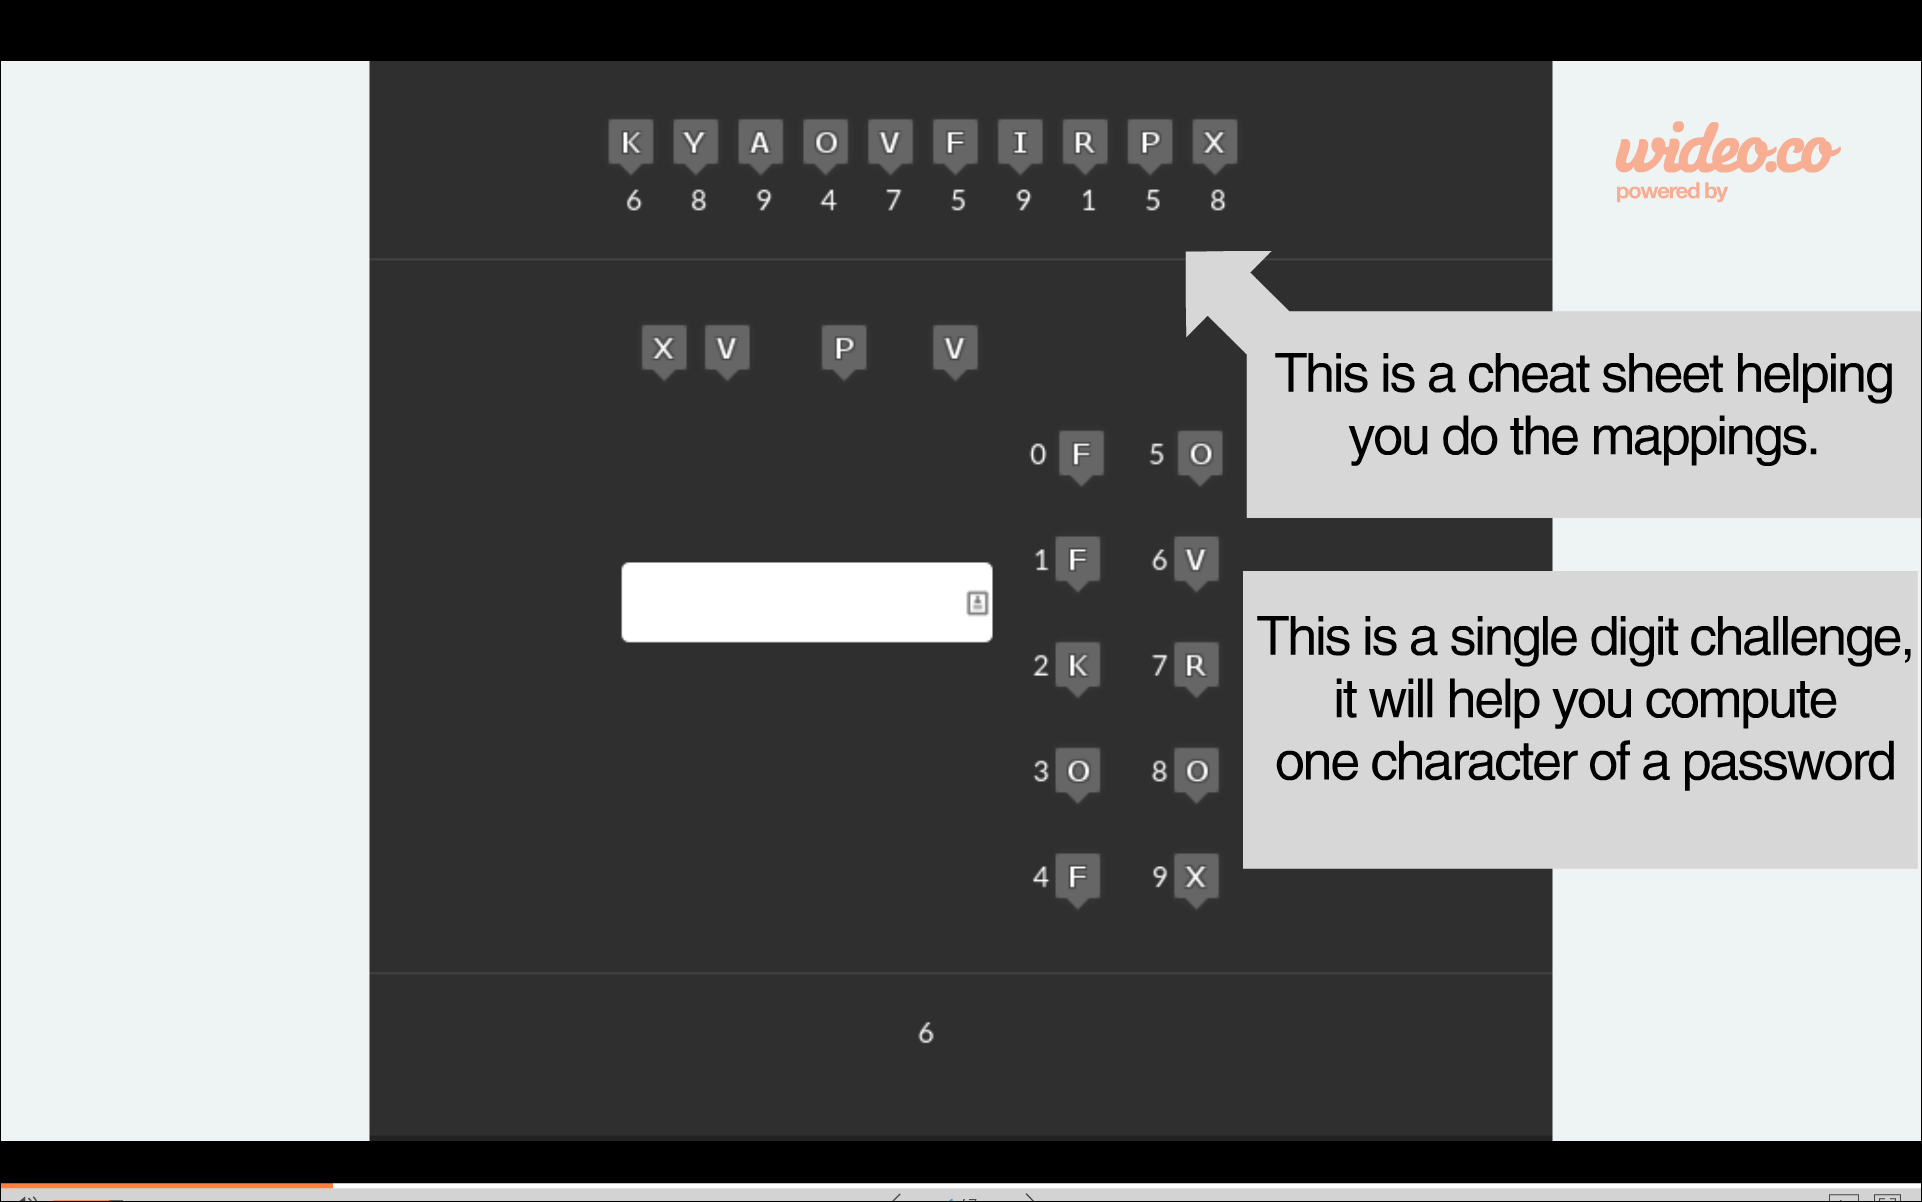
\includegraphics[width=\textwidth]{slides/slide1}
    \caption{Demo slide 1.}
    \label{slide1}
\end{figure}


\begin{figure}
    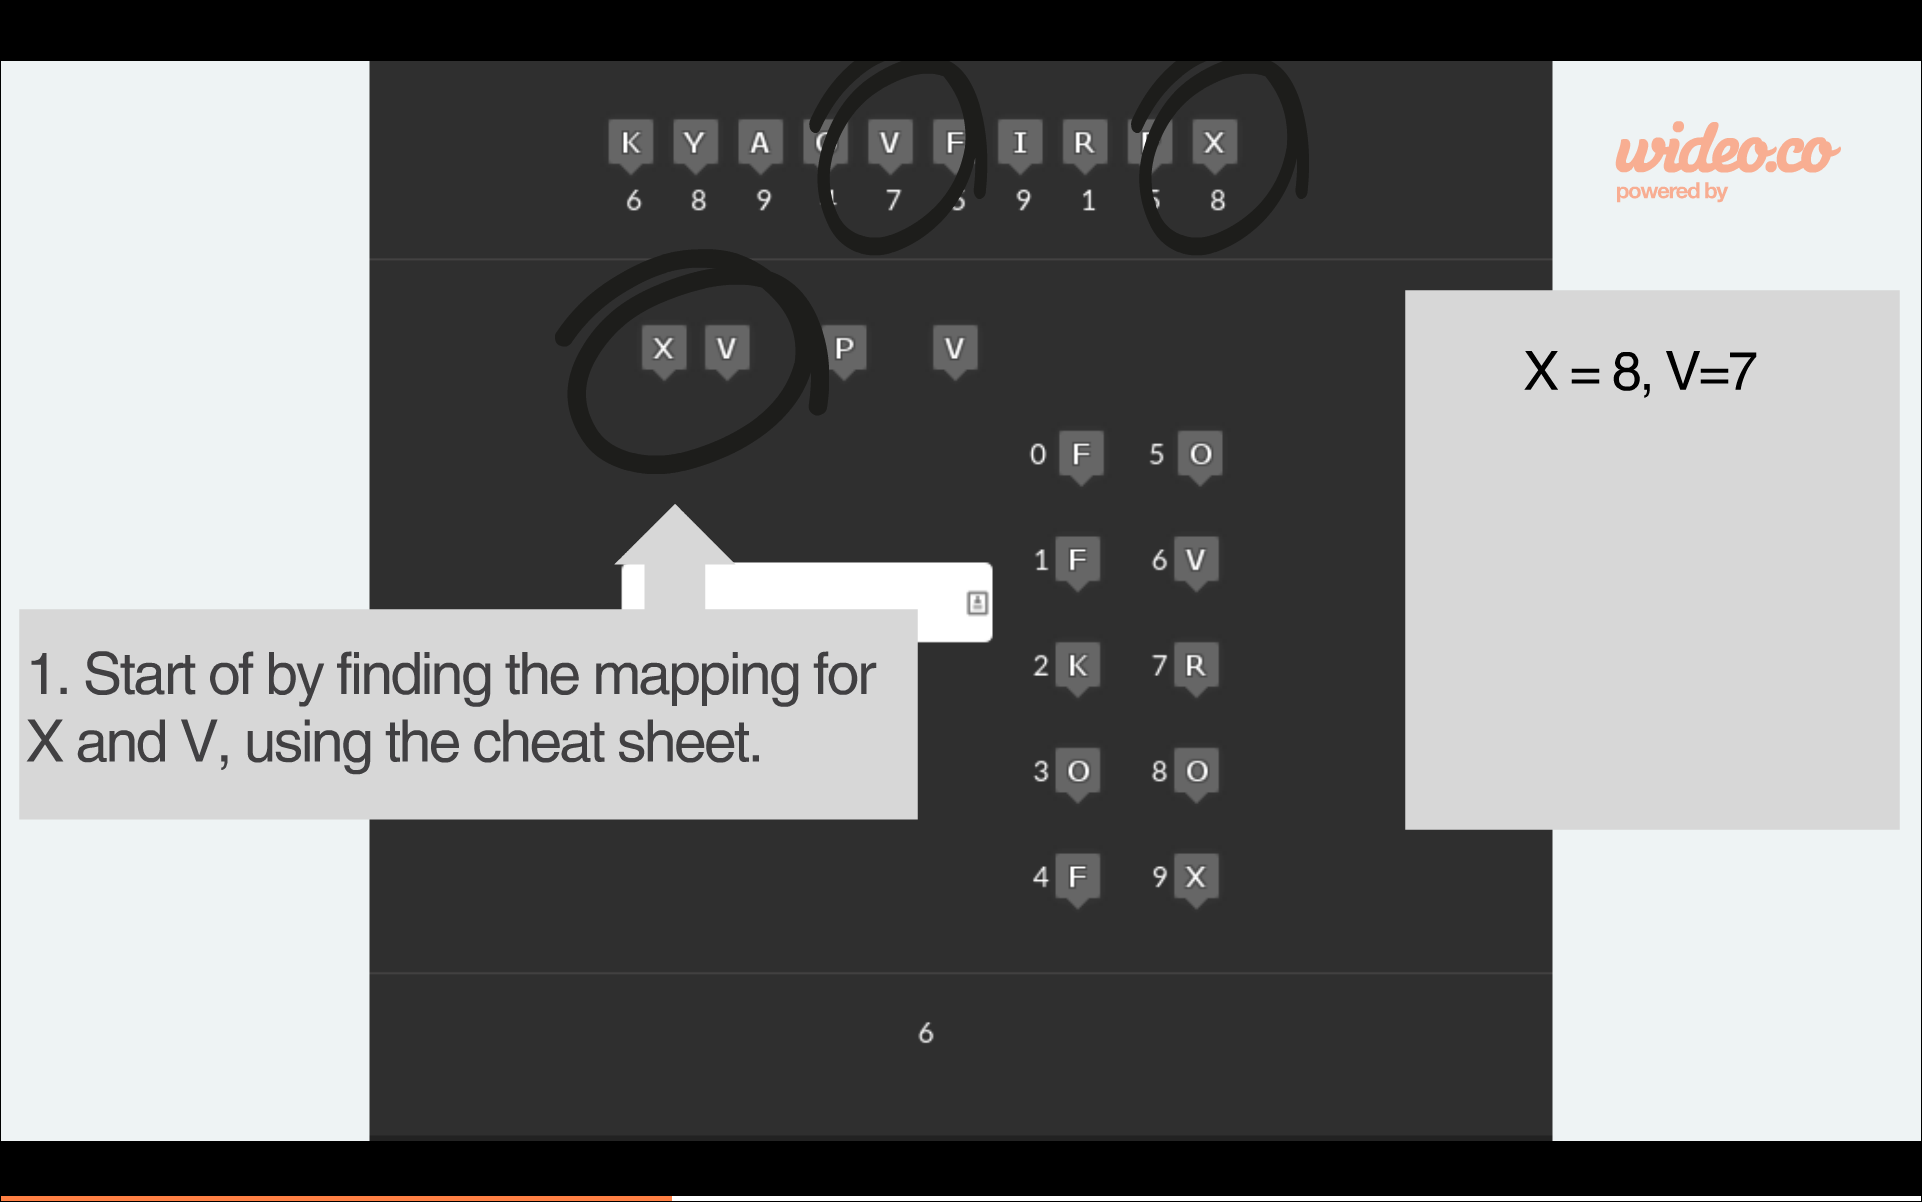
\includegraphics[width=\textwidth]{slides/slide2}
    \caption{Demo slide 2.}
    \label{slide2}
\end{figure}


\begin{figure}
    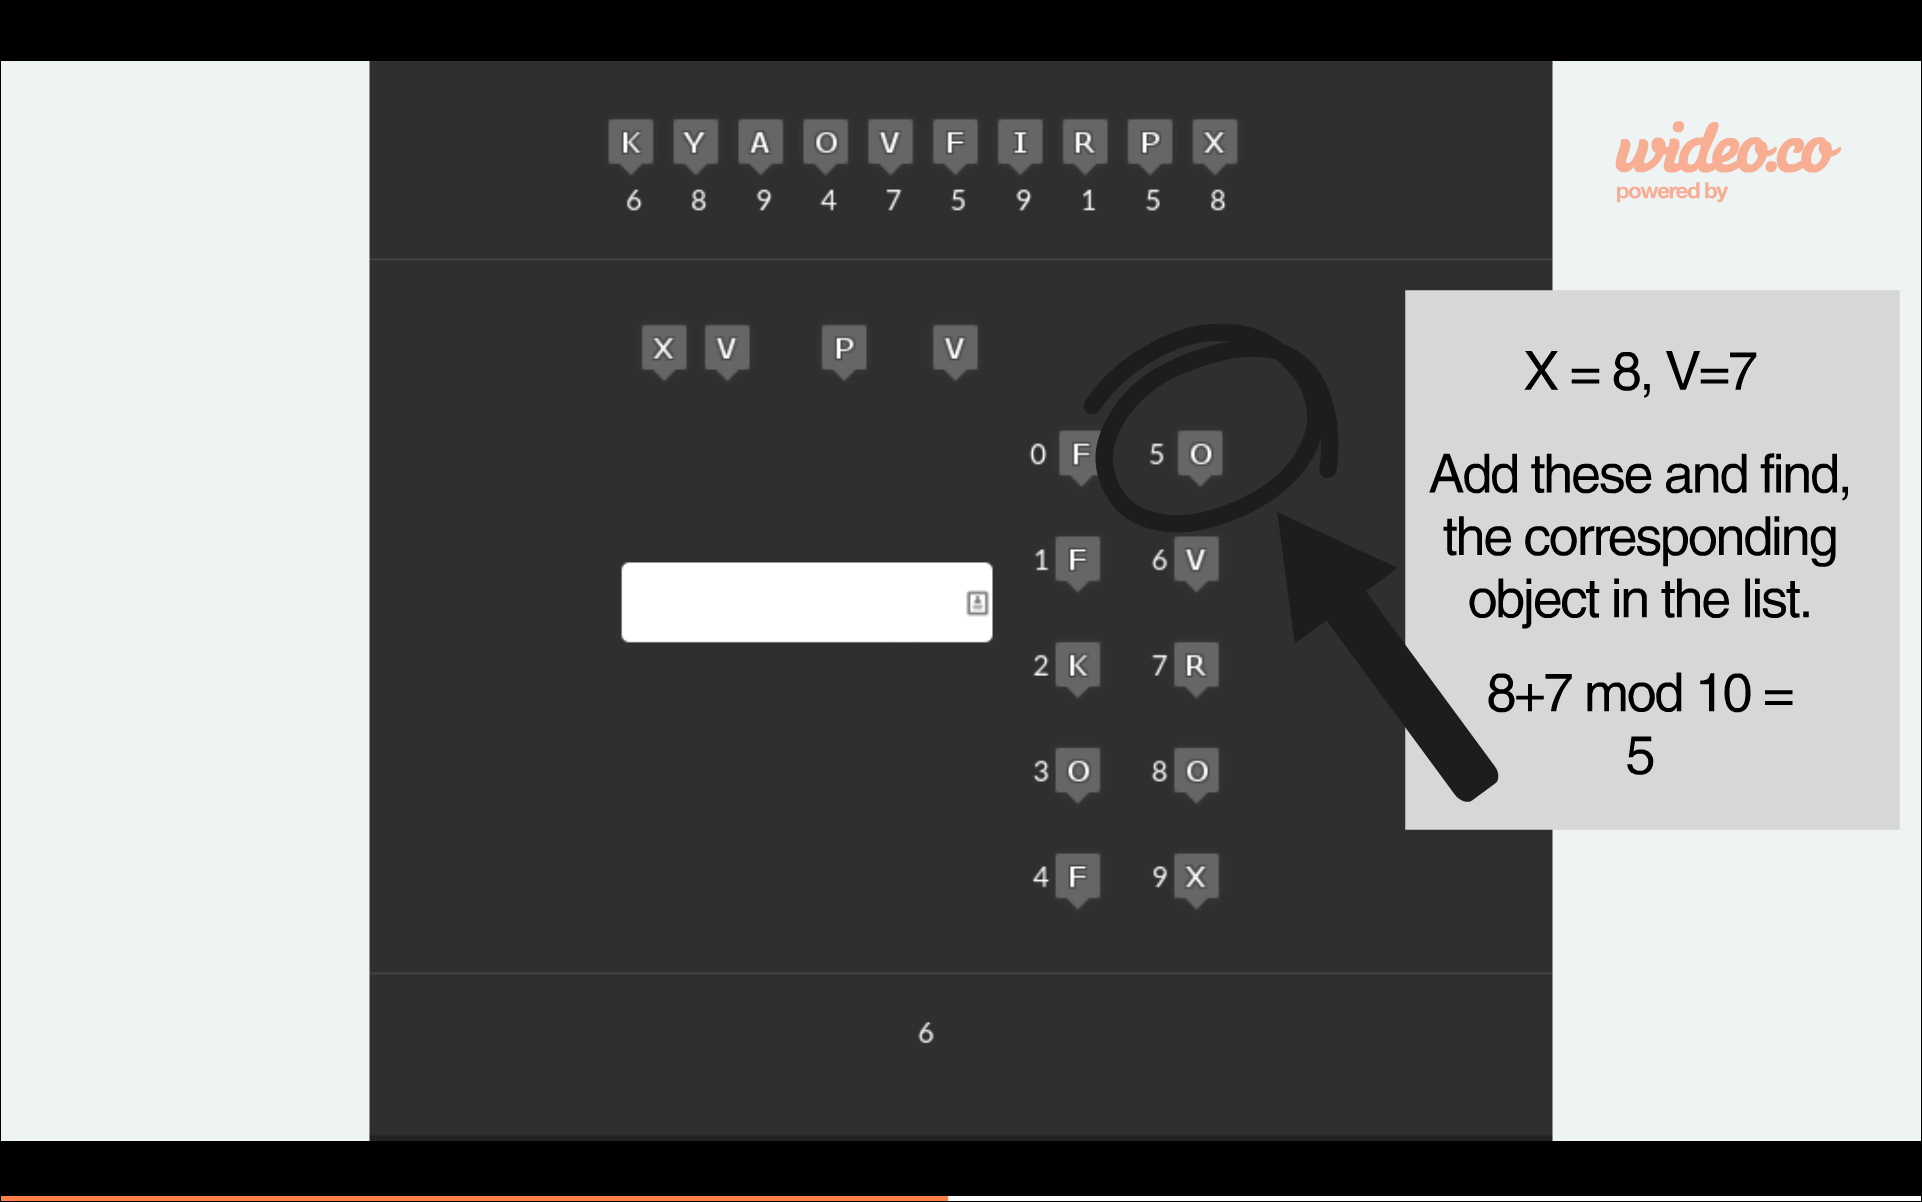
\includegraphics[width=\textwidth]{slides/slide3}
    \caption{Demo slide 3.}
    \label{slide3}
\end{figure}


\begin{figure}
    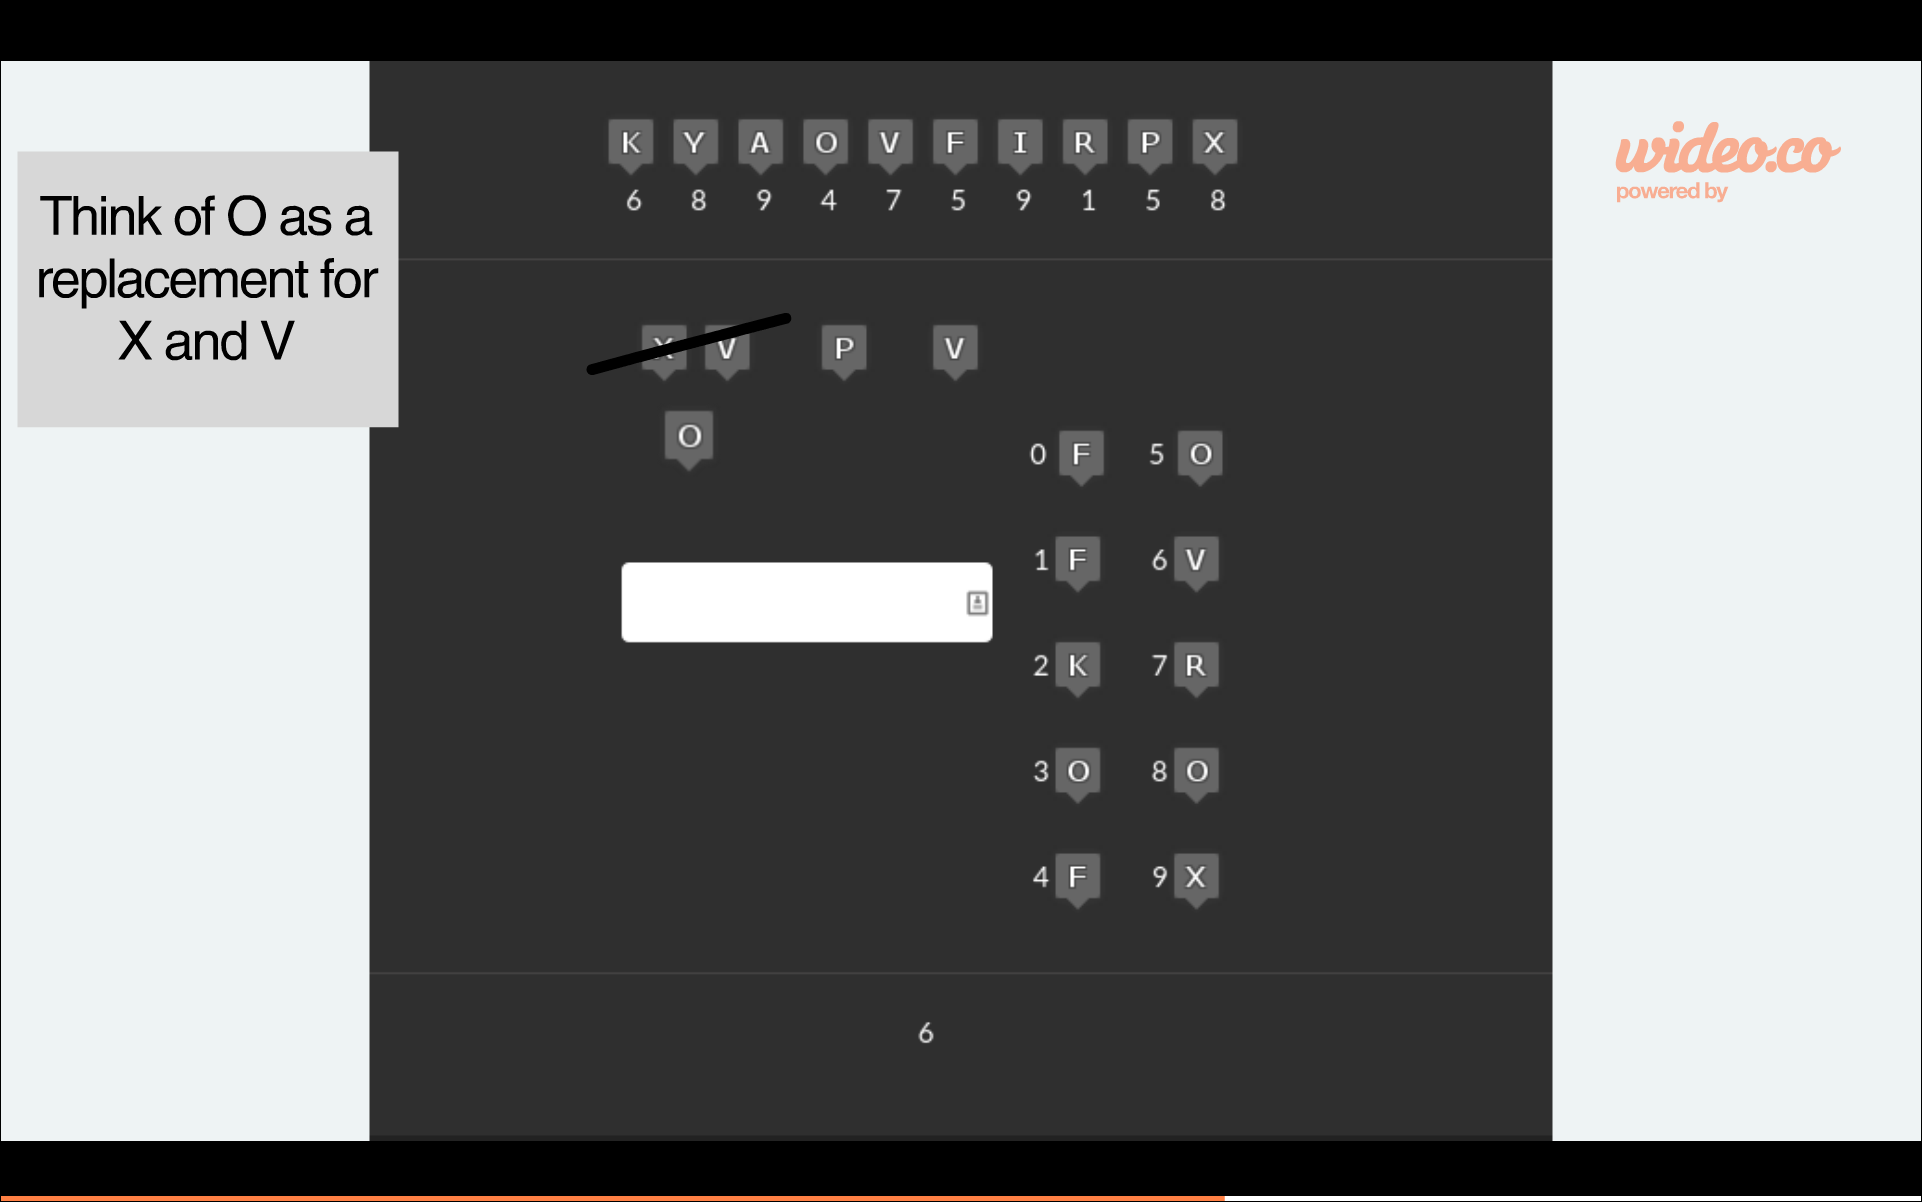
\includegraphics[width=\textwidth]{slides/slide4}
    \caption{Demo slide 4.}
    \label{slide4}
\end{figure}

\begin{figure}
    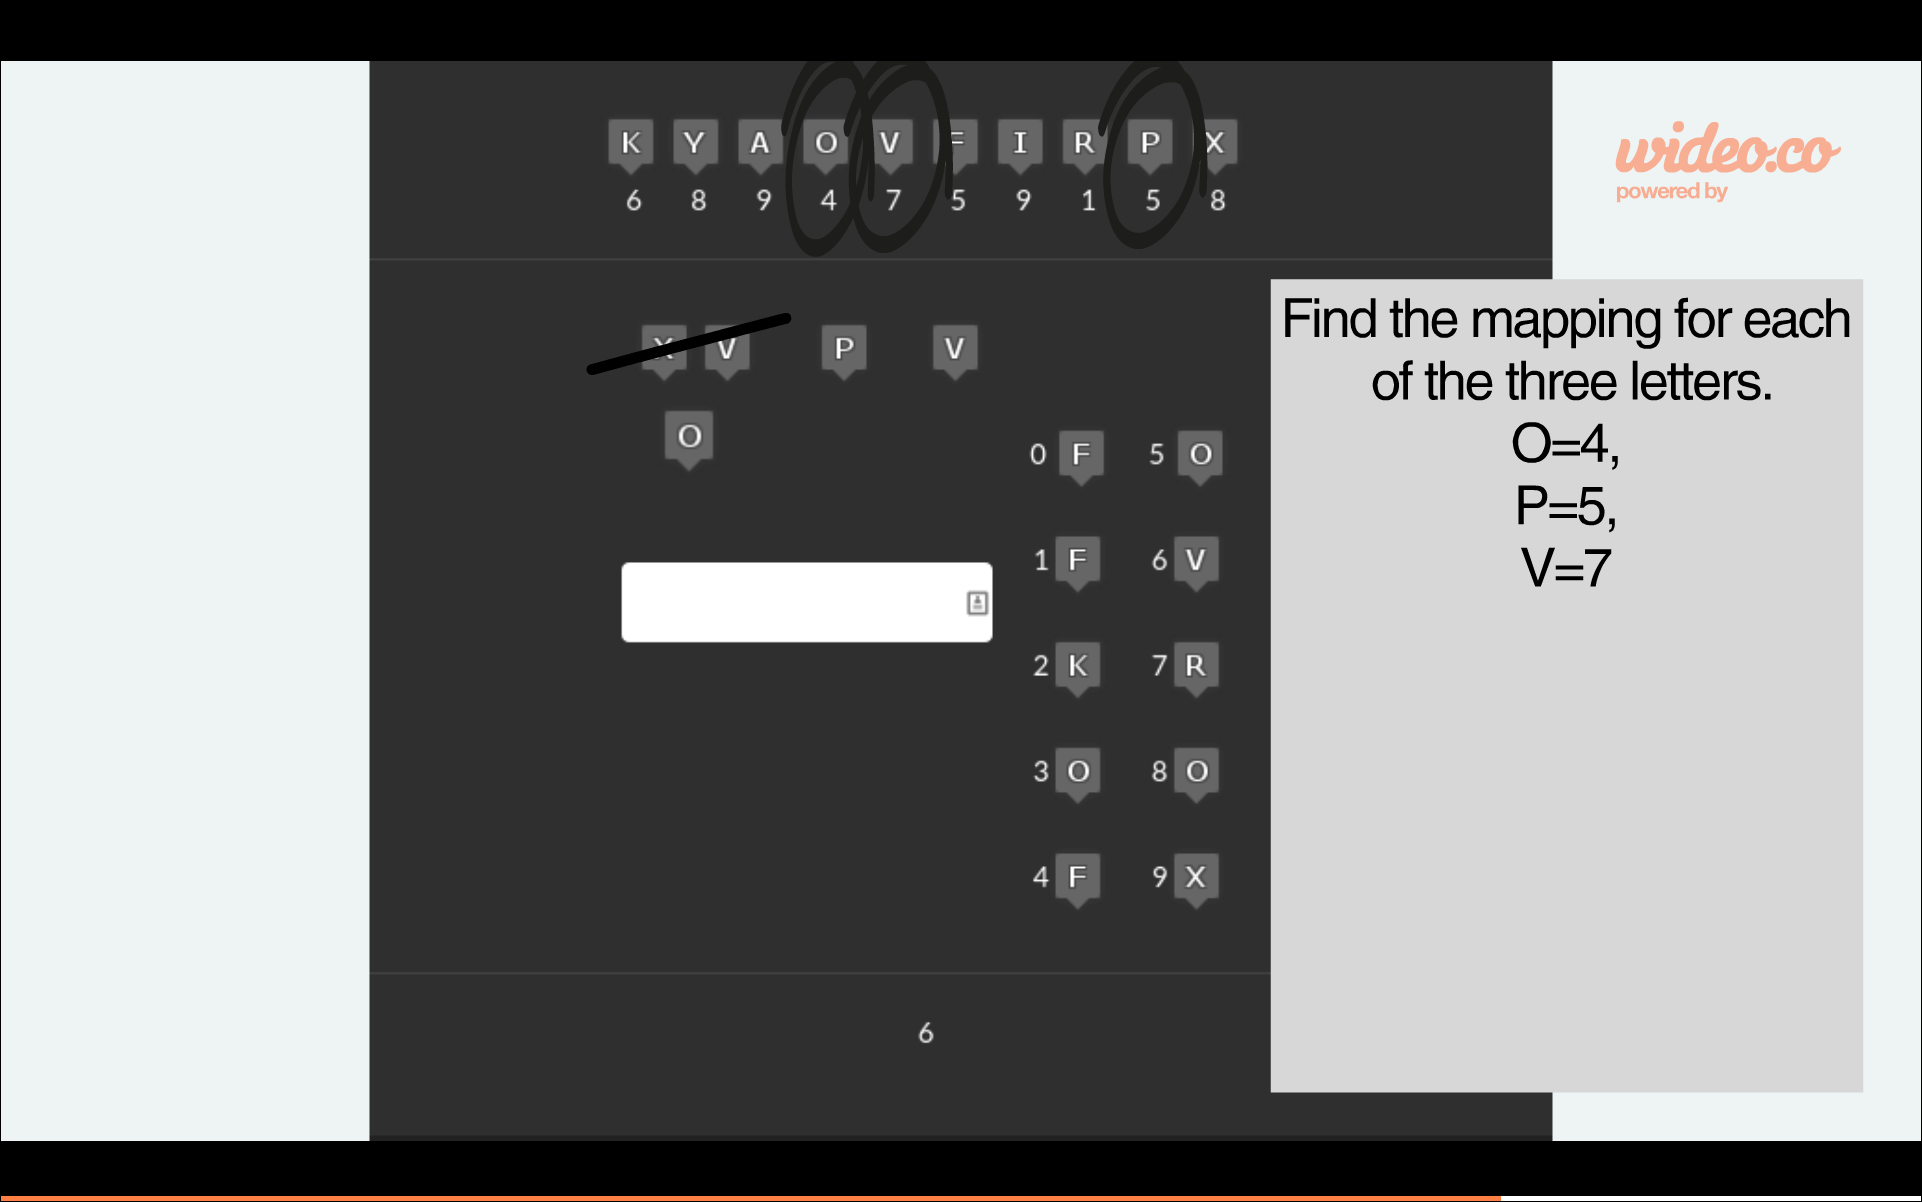
\includegraphics[width=\textwidth]{slides/slide5}
    \caption{Demo slide 5.}
    \label{slide5}
\end{figure}


\begin{figure}
    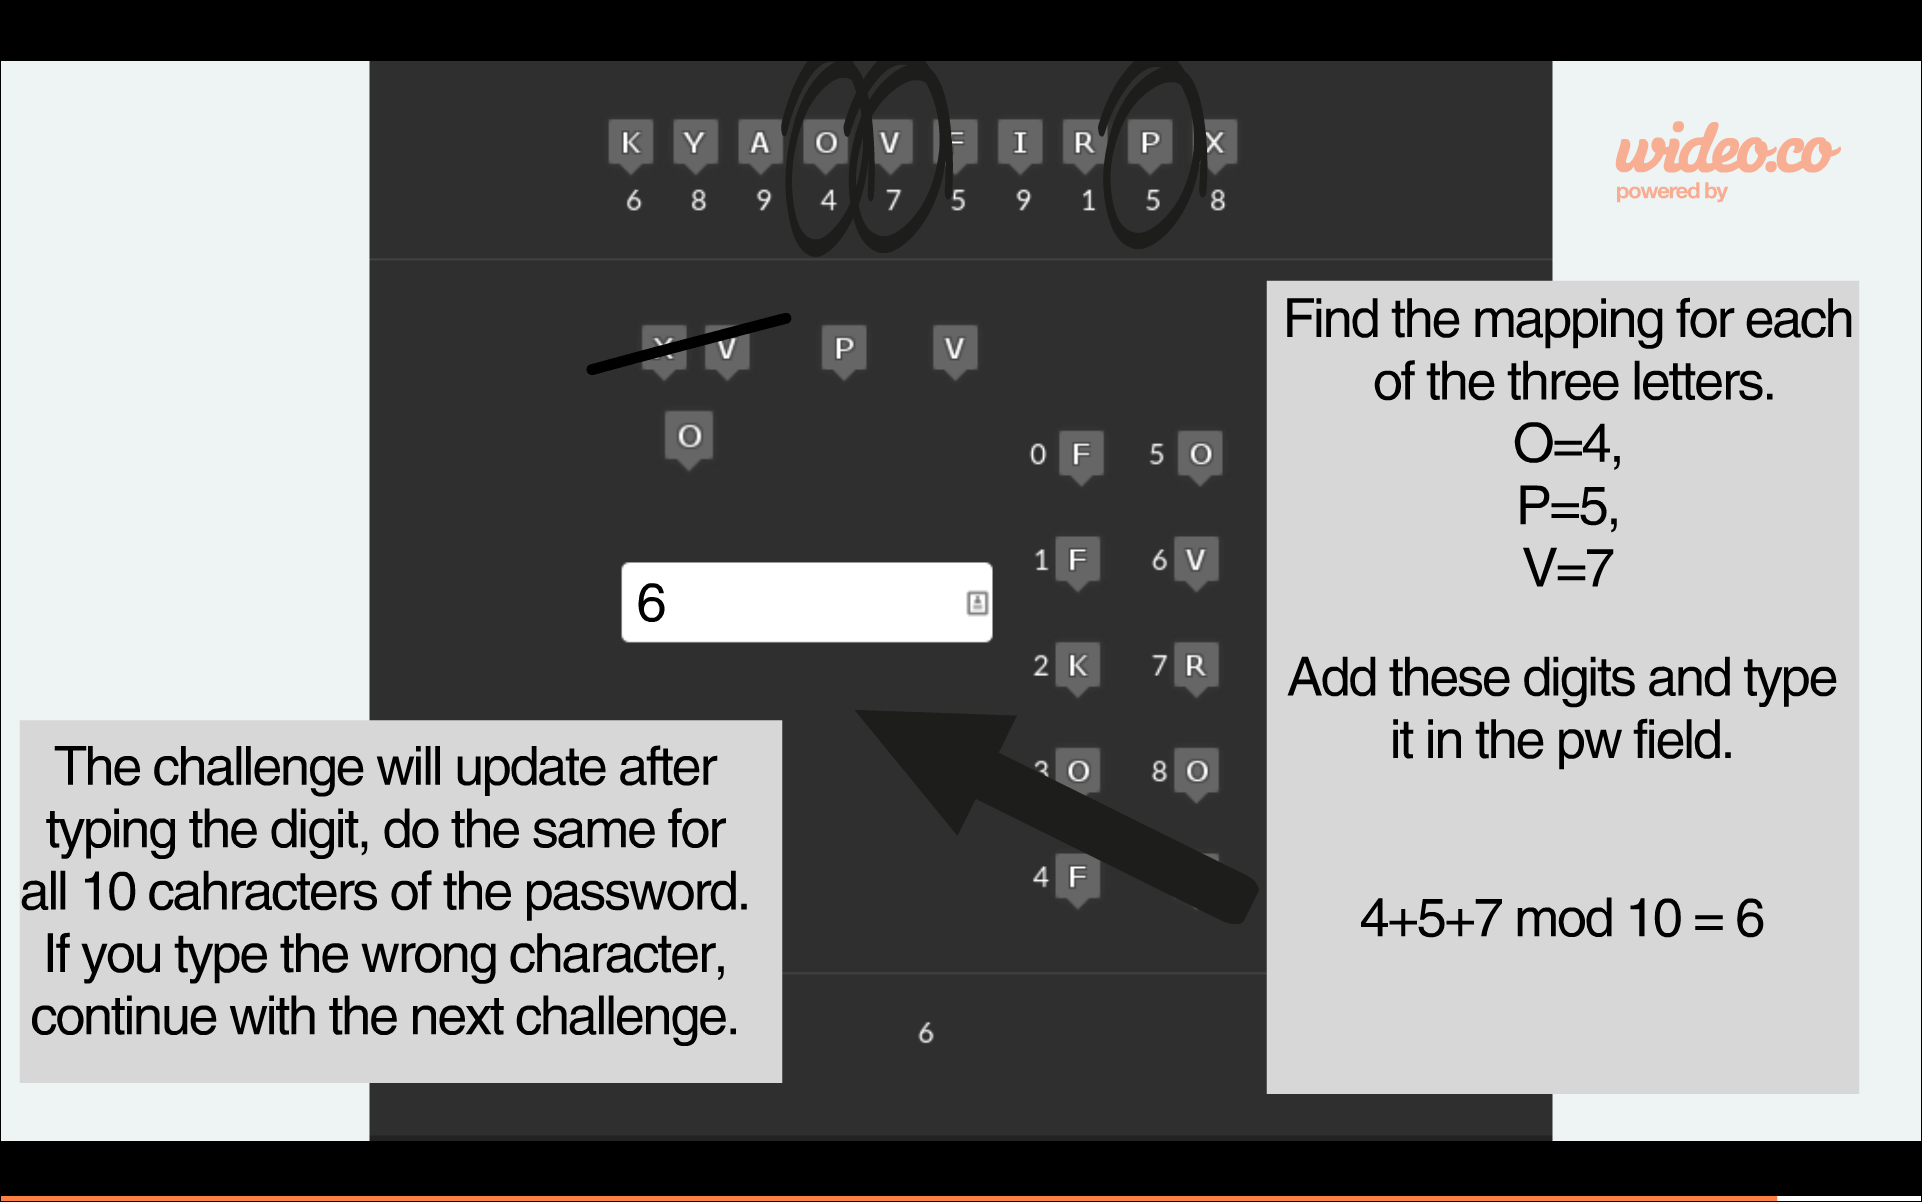
\includegraphics[width=\textwidth]{slides/slide6}
    \caption{Demo slide 6.}
    \label{slide6}
\end{figure}


\chapter{Extension class files}\label{extension-classes}

\section{Content Script}\label{app:content-script}
\lstinputlisting[caption=Content script file., style=jsStyle, basicstyle=\scriptsize]{code/content_script.js}

The content script listens for the onload event triggered by the windows object when a new page is loaded. When receiving this event the updateUrl function(line 27) is called, which sends an update containing the \emph{window.location.hostname} which essentially is the hostname of the current page. Hostname is used since login forms may be located at different locations at different domains.
\par Next the script search the DOM for input fields of type "password" using the \emph{getPwdInputs} function(line 16). This function iterates through all the input fields looking for password fields. If a password field is found, an event listener is attached to the field, listening for events of type "input" which are sent when the field changes\footnote{https://developer.mozilla.org/en-US/docs/Web/API/EventTarget/addEventListener}. When the password field changes a message containing the new length of the password is sent to the controller. 

\section{Controller}\label{app:controller}
\lstinputlisting[caption=Angular controller., style=jsStyle, basicstyle=\scriptsize]{code/controllers.js}

\section{App.js file}\label{app:app.js}
\lstinputlisting[caption=Angular launcher file., style=jsStyle, basicstyle=\scriptsize]{code/app.js}

\section{View file (partial file)}\label{app:view}
\lstinputlisting[caption=Angular view. Only included the table showing the challenges for readability., style=jsStyle, basicstyle=\scriptsize, firstline=32, lastline=91]{code/content.html}
